\frame{
    \frametitle{Finding a Basis with a Better Metric}
        \begin{columns} \begin{column}{0.4\textwidth}
    \begin{center} 
        (70 Possible Combinations of 6... 30 if requiring SM point)

        \resizebox{0.3\textheight}{!}{\begin{tabular}{ |l|l|l| }
            \hline
                \textbf {$\kappa_{2V}$} & \textbf {$\kappa_\lambda$} & \textbf {$\kappa_V$} \\
                \hline
                \rowcolor{red}   0   & 0   & 1   \\ % !!
                0   & 1   & 1   \\ 
                0.5 & 1   & 1   \\ 
                1   & 0   & 1   \\ 
                \rowcolor{red}   1   & 1   & 0.5 \\ % !!
                1   & 1   & 1   \\ 
                \rowcolor{red}   1   & 1   & 1.5 \\ % !!
                1   & 10  & 1   \\ 
                1   & 2   & 1   \\ 
                1.5 & 1   & 1   \\ 
                2   & 1   & 1   \\ 
                4   & 1   & 1   \\ 
                \rowcolor{green} 0   & 1   & 0.5 \\ % !!
                \hline
                \end{tabular}} \end{center}
    \end{column} \begin{column}{0.5\textwidth}

    {\small
        I don't trust the ``Hash-Max" measure of performance anymore, for reasons that will soon be clear.

        I think have a better metric of performance now.
    }

    \begin{figure}
    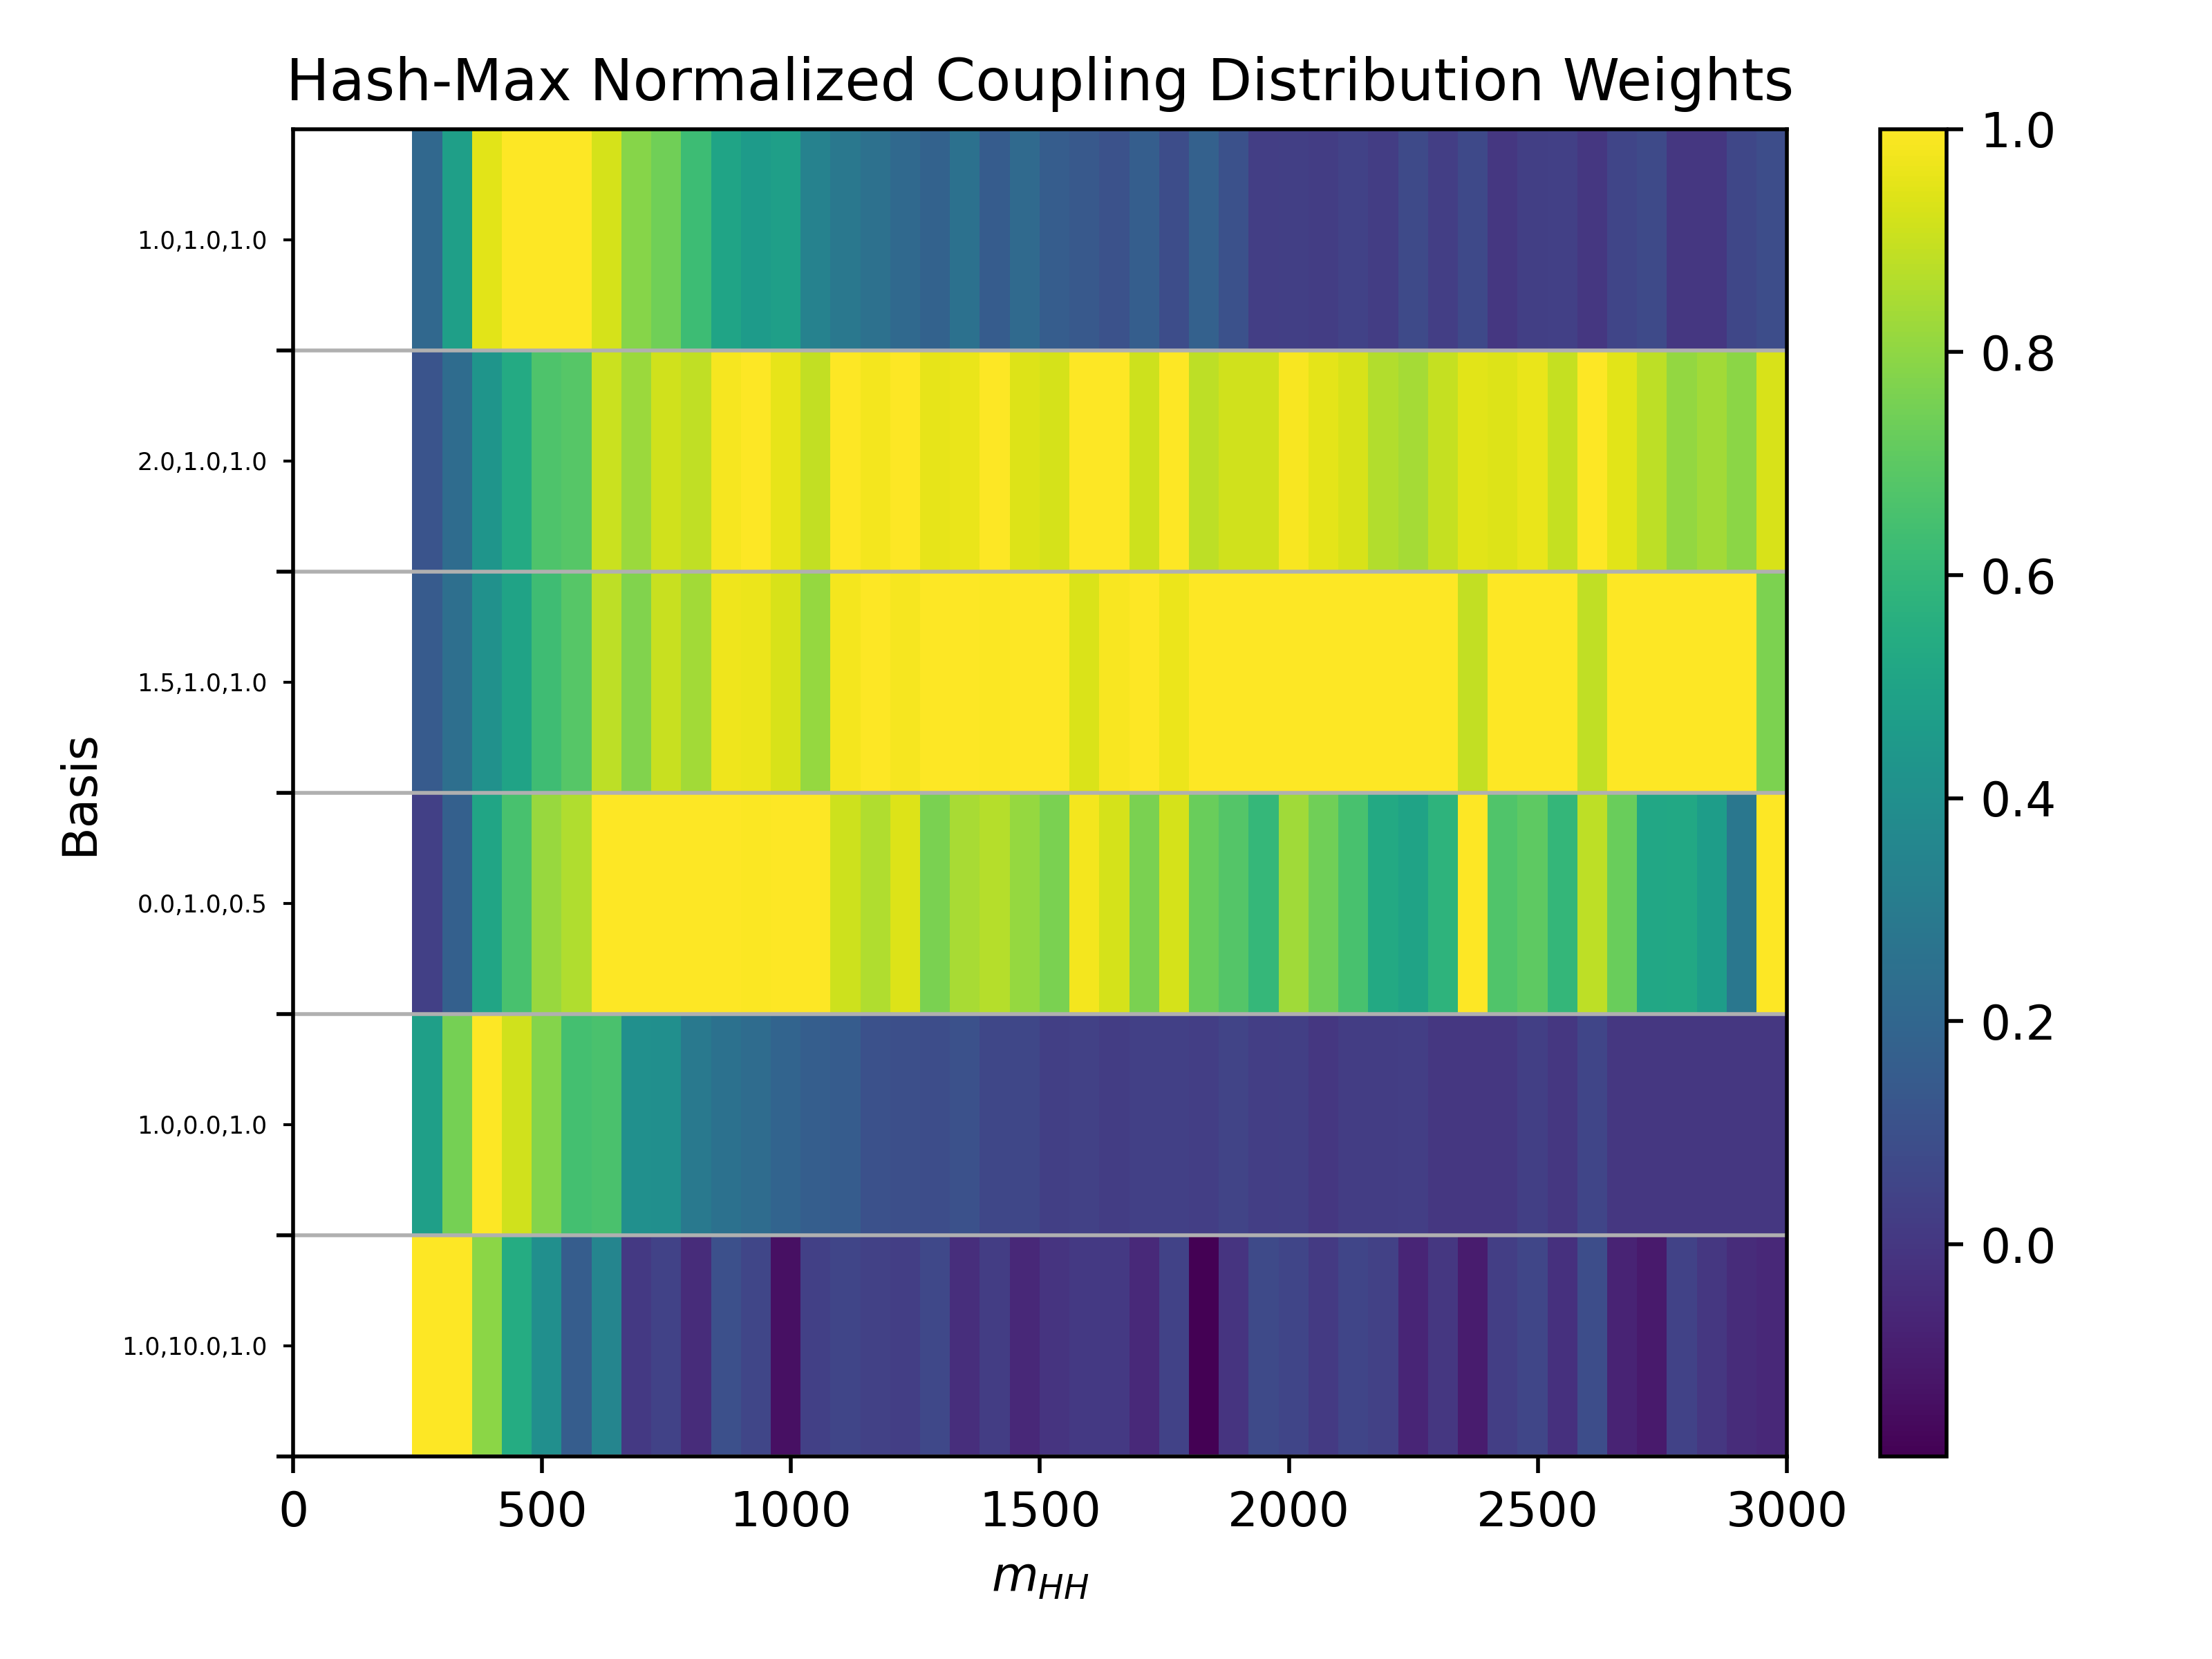
\includegraphics[width=\linewidth,height=\textheight,keepaspectratio]{coupling_scan_auto_chosen_reco_R0_hash_max}
    \end{figure}
    \end{column} \end{columns}
}

\displayonelarge{Negative Weights}{
    Negative weights can appear in the $m_{HH}$ combination. These are unphysical and should be avoided.
}{reco_mHH_cvv1p0cl2p0cv1p0}

\displayonelarge{Extreme Negative Weights}{
    In further regions of the $\kappa$ parameter space, these negative weights can be become dangerously common.
}{preview_reco_mHH_cvv0p0cl-9p0cv1p0_old}

\displayonelarge{Ranking Basis by Negative Weight Integral}{
    Take the surface integral of the number of negative bins at each point at in the $\kappa$ parameter space (mutliplying by the $\kvv \times \kl$ ``area")
}{negative_weights_rank027}

\displaythree{Negative-Weight Map of Different Bases}{
    Other bases show considerable improvement in the number of negative bins
}
{negative_weights_rank027}
{negative_weights_rank015}
{negative_weights_rank000}

\displayonelarge{Minimal Negative Weight Basis}{
    \begin{center} 
        \resizebox{0.3\textheight}{!}{\begin{tabular}{ |l|l|l| }
            \hline
                \textbf {$\kappa_{2V}$} & \textbf {$\kappa_\lambda$} & \textbf {$\kappa_V$} \\
            \hline
                1   & 1   & 1   \\ 
                0   & 1   & 0.5 \\
                1   & 0   & 1   \\ 
                1   & 10  & 1   \\ 
                0.5 & 1   & 1   \\ 
                4   & 1   & 1   \\ 
            \hline
    \end{tabular}} \end{center}
}{negative_weights_rank000.png}

\displayfour{Using Minimal Negative Weight Basis}
{reco_mHH_cvv1p0cl2p0cv1p0}
{reco_mHH_new_cvv1cl2cv1}
{preview_reco_mHH_cvv0p0cl-9p0cv1p0_old}
{preview_reco_mHH_new_cvv0cl-9cv1}


\displaytwocaption{Limits with Negative-Weight Integral Rank-1 Basis}{
    Fewer negative weights results in a much more ``natural" limit boundary.

    Sharp edges and corners appear to have been a consequence of poor signal modelling.
}
{2D_scan_2D_scan_test01_noMC16e_samps_vbf_pd_1617_c1v1.0_exclusion}
{Using old basis}
{2D_scan_2D_scan_test02_newBasis_samps_vbf_pd_1617_c1v1.0_exclusion}
{Using new basis}
